\documentclass[a4paper,12pt]{article}
\setlength{\parskip}{0.5pt}%
\setlength{\parindent}{20pt}%

%preamble: style and/or packages
\author{Hanyi Jiang}
\title{Research proposal}
\date{January 2023}

%\usepackage{package}

\usepackage{hyperref}
\usepackage{titlesec}
\setcounter{secnumdepth}{3}
\usepackage{enumitem}
\usepackage{varwidth}
\usepackage{tasks}

\usepackage{graphicx}
\usepackage{siunitx}
\usepackage{url}

%colors, boxes
\usepackage[dvipsnames]{xcolor}
\usepackage[most]{tcolorbox}
\tcbuselibrary{fitting}

\definecolor{columbiablue}{rgb}{0.61, 0.87, 1.0}
\definecolor{mossgreen}{rgb}{0.68, 0.87, 0.68}

\usepackage[super,sort&compress,comma]{natbib}
\bibliographystyle{naturemag}

%indent first line
\usepackage{indentfirst}
\setlength{\parindent}{30pt}

%captions
\usepackage[font=footnotesize,labelfont={bf,it}, textfont=it]{caption}
\usepackage[labelsep=period]{caption}

%landscape pages
\usepackage{pdflscape}
\usepackage{fancyhdr} 

%page number at bottom in landscape 
\fancypagestyle{mylandscape}{
\fancyhf{} %Clears the header/footer
\fancyfoot{% Footer
\makebox[\textwidth][r]{% Right
  \rlap{\hspace{.75cm}% Push out of margin by \footskip
    \smash{% Remove vertical height
      \raisebox{4.87in}{% Raise vertically
        \rotatebox{90}{\thepage}}}}}}% Rotate counter-clockwise
\renewcommand{\headrulewidth}{0pt}% No header rule
\renewcommand{\footrulewidth}{0pt}% No footer rule
}

%temporarily disable superscript
\DeclareRobustCommand*{\citen}[1]{%
  \begingroup
    \romannumeral-`\x % remove space at the beginning of \setcitestyle
    \setcitestyle{numbers}%
    \cite{#1}%
  \endgroup   
}


\begin{document}
	
	% cover page
	\begin{center}
	\thispagestyle{empty}
		\begin{LARGE}
		Mapping global STEM funding using AI  \\[1 cm] \vfill
		\end{LARGE}
			
			
		\begin{Large}
			Research proposal \\ [1 cm]\vfill
			Author \\
			\href{mailto:<email>}{Hanyi Jiang} \\[1 cm]\vfill
			
			
			April, 2023\\[1 cm]\vfill
			
			Supervisor: Dr Samraat Pawar \\ 
			\vfill
			
			Department of Life Sciences  \\
		
            
			
		\end{Large}
	\end{center}
	
	% document begins
	\newpage
    \section{Keyword}
    Funding organization, Research grant

    \section{Introduction}
	Hand in hand with the rise of New Public Management and expanding global techno-economic competition, increasing prominence has been given to the idea that countries have been paying more attention on research project over the last 20 years. \cite{sargent2017global} The two most important components of any research project is idea and execution. The successful execution of the research project depends not only on the effort of the researcher but also on the available infrastructure to conduct the research. The conduct of a research project entails expenses on man and material and funding is essential to meet these requirements. \cite{neema2021research} Therefore, the funding largely influences the project's progress. In this project, we will focus on the direction of funding to find the change in the focus of the academic committee over time in UK and US. Then the results are used to analyze the differences in subject priorities between the two countries. \\
    ~\\
    \indent This project aims to answer the following questions: \\
    \indent 1. Whether and if so, exactly how the core subjects and STEM priorities of governments have changed over time? \\
    \indent 2. Do the STEM priorities of governments in the UK and the US overlap at the same point in time?\\
    

	\section{Method}
    
    I already have the pre-processed clean data which contains information such as project title, abstract, and funding amount, so I can spend a short time double-checking to make the data specifically fit my focus.\\

    Topic models provide a simple approach to analyze huge volumes of unlabeled text. \cite{jelodar2019latent}Through topic analysis, we can analyze the content of successful grant proposals to find common themes in large collections of text. Then fit and train LDA model to model research topics to get the result of topic probabilities for each document, which is a quantitative measure of dominant themes for each document. The hyperparameters $\alpha$ (alpha) and $\beta$ (beta) are involved in this step.\cite{Topic-Analysis:-The-Ultimate-Guide-https://monkeylearn.com/topic-analysis/} Finally, after identifying topics across all the funded projects, we can quantify how funding has been allocated across the topics in each year in UK and US. This analysis consisted of four steps: (1) calculating total funding in each year in UK and US (2) comparing received funding in each topic (3) listing the top 10 subject priorities in each year in both UK and US and labeling all topics using the Library of Congress Classification Outline as a guide. 
    \\



	\section{Anticipated Outcomes}
	For the first question, the best-case scenario is that some specific subjects consistently at the top of the rankings, some subjects from the top change to the middle of the list, or some subjects list position change from bottom to the top. However, sometimes it may not be such easy, if we cannot find the change of the subjects, some other analysis may need. \\
    \indent For the second question, the top 10 subject priorities of UK and US should overlap to a large extent. If time permits, we can analyze in a more in-depth way to quantify in a statistical perspective.\\
	
	\section{Time Line}
	\noindent
    Month 1: Reading and finding resources, Writing Introduction\\
    Month 2-3: Parameterizing models\\
    Month 4-5: Analysis and writing\\

	\begin{figure}[htbp]
		\centering 
		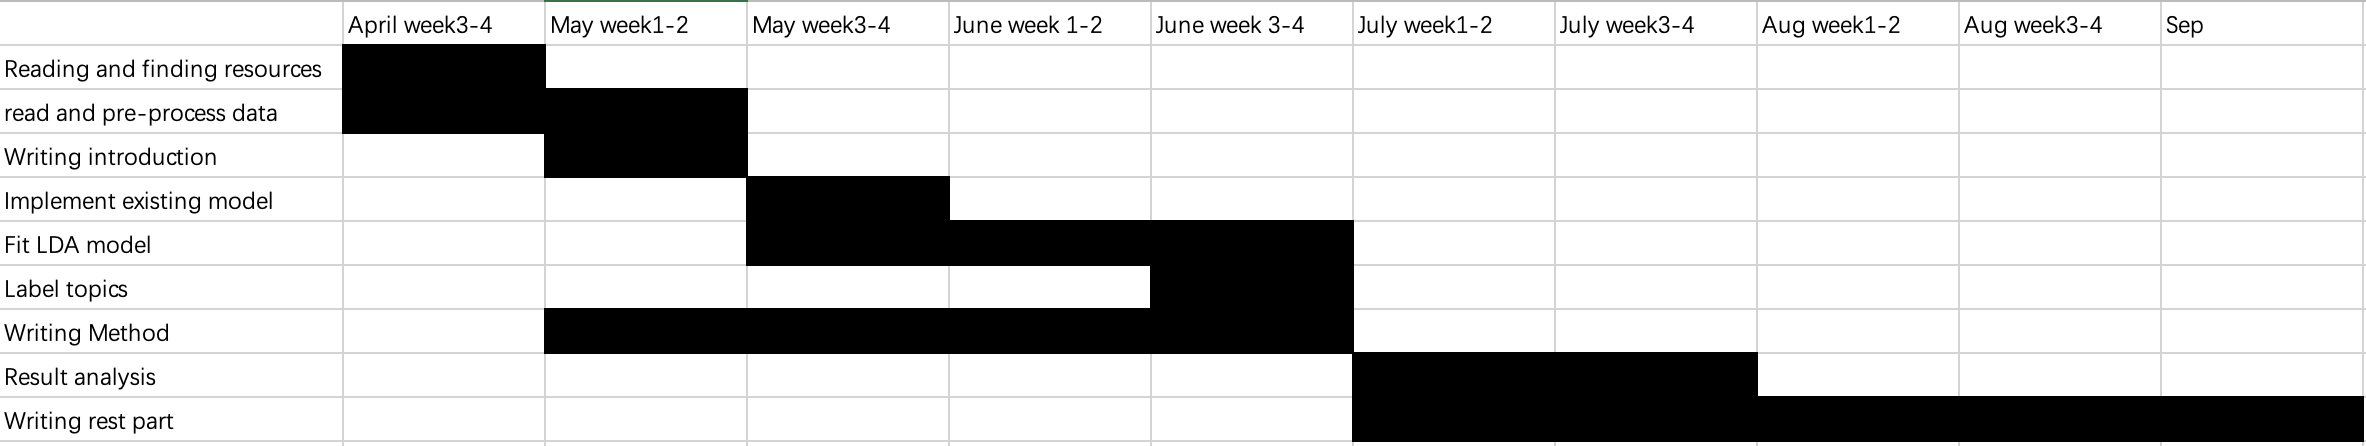
\includegraphics[width=1.1\textwidth]{timetable.jpeg} 
		\caption{Estimate Timetable}
		\label{Fig.main2}
	\end{figure}




\bibliographystyle{plain}
  
\bibliography{Research_Proposal}





\end{document}